% !TEX root = ../notes_template.tex

\chapter{코시 적분 정리와 응용}

복소미분은 어느정도 익숙해졌으니 이제 적분으로 관심을 돌려보자.
이 장에서는 복소해석학에서 매우 중요한 다음 정리를 배울 예정이다.
\begin{center}
\fbox{
코시 적분 정리
}
\end{center}
``경로적분''을 정의하는 것으로 시작하여 나중에 코시 적분 정리를 증명할 예정이다.
왜 경로적분과 코시 적분 정리가 왜 그렇게 중요한지 의문을 가질 수 있다.
복소평면에서 적분의 중요성은 복소해석함수의 더 큰 이해로 이어지기 때문이다.
예를 들면, 복소해석함수는 무한번 미분가능하다는 본질적인 성질이 있다.
이 장에서 다음 주제들을 중심으로 공부해보기로 하자.
\begin{enumerate}
\item[(1)] 경로적분의 정의와 성질
\item[(2)] 경로적분의 기본정리
\item[(3)] 코시 적분 정리
\item[(4)] 코시 적분 정리의 응용
\begin{enumerate}
\item 부정적분의 존재성
\item 복소해석함수의 무한번 미분가능성
\item 리우비우 정리와 대수학의 기본정리
\item 모레라 정리
\end{enumerate}
\end{enumerate}

\section{경로적분의 정의}

일반적인 미적분에서 연속함수 $f: [a,b] \to \mathbb R$가 주어질 때
\begin{equation}\label{eq-3-1}
\int_a^b f(x)dx
\end{equation}
의 의미는 명확하다. 이제 이를  일반화하여 복소수까지 확장하고
주어진 복소수 $z$, $w$에 대하여
\[
\int_z^w f(\zeta)d\zeta
\]
에 의미를 부여하길 원한다고 하자.
$z$에서 $w$까지를 어떻게 해석해야 할까?

$\mathbb R$에서 $a<b$이면, 실수 $a$부터  실수 $b$까지
가는 경로는 한가지 뿐이다.  
따라서 실수의 경우는 단지
\begin{itemize}
\item[(1)] $a<b$이고,
\item[(2)] 연속함수 $f:[a,b] \to \mathbb R$
\end{itemize}
의 경우만 생각하면 충분하다.

하지만, $z$와 $w$가 복소평면 위의 점이면
그림 \ref{fig-3-1}과 같이 많은 경로에 대하여 적분을 생각할 수 있다.

\begin{figure}[!h]
\begin{center}
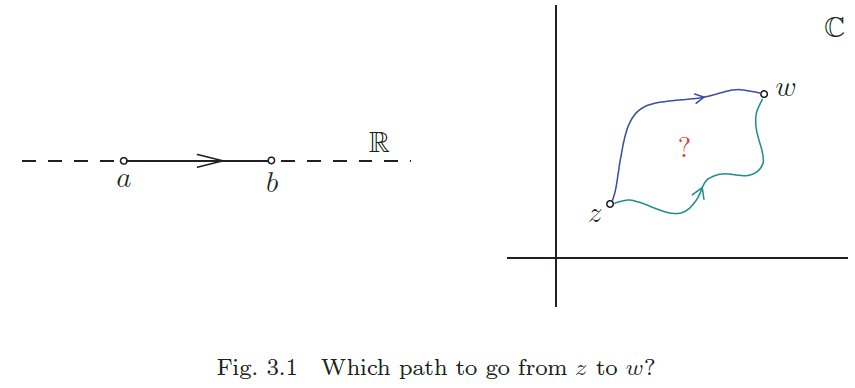
\includegraphics[width=0.8\textwidth]{./SaltChapter/fig-3-1}
\end{center}
\caption{$z$에서 $w$까지 어떤 경로로 가야할까?}
\label{fig-3-1}
\end{figure}

그러므로 복소수의 경우는 끝점 $z$와 $w$ 외에
$z$에서 $w$까지의 경로 $\gamma$도 지정하고,
실수의 경우를 나타낸 식 \eqref{eq-3-1}를
다음과 같이 복소수에 대한 표현으로 바꾸도록 한다.
\[
\int_\gamma f(z)dz.
\]

이 표현을 ``경로''적분이라 부르며
계산을 위해 다음을 정할 필요가 있다.
\begin{itemize}
\item[(1)] 정의역  $D(\subset \mathbb C)$와 $z, w\in D$
\item[(2)] 연속함수 $f:D\to \mathbb C$
\item[(3)] $z$와 $w$를 잇는 매끄러운 경로 $\gamma: [a,b] \to D$
\end{itemize}

